\documentclass{beamer}
\usetheme{metropolis}
\usepackage{graphicx}
\usepackage{subfig}
\title{Safe Return Doubtful: Week 3 part I}
\date{\today}
\author{Jordan Hanson}
\institute{Whittier College Department of Physics and Astronomy}

\begin{document}
\maketitle

\section{Summary}

\begin{frame}{Summary}
\begin{enumerate}
\item Summarize force, work, and vectors required to move in Antarctica
\begin{itemize}
\item $\vec{d} = d_x\hat{x}+d_y\hat{y}$
\item $h = \sqrt{d_x^2 + d_y^2}$
\item $d_x = h\cos(\theta)$, $d_y = h\sin(\theta)$
\item $F_f = \mu m g$ (force of friction)
\item $W = Fd$ (work)
\item $W = \mu m g d$ (work specific case of friction)
\item $F = mg$ (force of gravity)
\item $W = mgd$ (work required to raise altitude)
\item \textbf{3D: terrain (different frictions) and \textit{elevation}}
\end{itemize}
\item \textbf{Activity: navigation through terrain}
\item Introduction to Radio-glaciology
\end{enumerate}
\end{frame}

\section{Summary of force, work, and vector navigation}

\begin{frame}{Summary of force, work, and vector navigation}
\begin{equation}
\vec{d} = d_x\hat{x}+d_y\hat{y}
\end{equation}
\begin{align}
d_x &= h\cos(\theta) \\
d_y &= h\sin(\theta)
\end{align}
Imagine your expedition begins at the origin of an x-y coordinate system.  You head West for 15 km, and then 45 degrees North of West for 15 km.  What is your final position in x-y space? Draw a sketch of this trajectory.  (\textbf{Work this one at your tables.})
\end{frame}

\begin{frame}{Summary of force, work, and vector navigation}
\begin{equation}
\vec{d} = d_x\hat{x}+d_y\hat{y}
\end{equation}
\begin{align}
d_x &= h\cos(\theta) \\
d_y &= h\sin(\theta) \\
\theta &= tan^{-1}(\theta)
\end{align}
Same situation, what is your current distance from the origin?  What angle are you making with the x-axis (what is your heading)?  (\textbf{Work this one at your tables.})
\end{frame}

\begin{frame}{Summary of force, work, and vector navigation}
\begin{equation}
F_f = \mu m g
\end{equation}
Suppose you are traveling on snow, and the coefficient of friction is $\mu = 0.05$ between the sled carrying your cargo and the snow.  The cargo has a mass of 500 kg.  How much force is required to pull it against friction? (g = 9.81 m/s$^2$).  (\textbf{Work this one at your tables.})
\end{frame}

\begin{frame}{Summary of force, work, and vector navigation}
\begin{equation}
W = \mu m g d
\end{equation}
Same situation.  You have 10 sled dogs, each of whom can pull with a force of 50 Newtons.  If each dog pulls with 50 Newtons, will the sled move?  What is the minimum force with which the sled dogs must pull to move the sled?  (\textbf{Work this one at your tables.})
\end{frame}

\begin{frame}{Summary of force, work, and vector navigation}
\begin{equation}
W = \mu m g d
\end{equation}
Same situation.  You have 10 sled dogs, each of whom can pull with a force of 50 Newtons.  If each dog pulls with 50 Newtons, will the sled move?  What is the minimum force with which the sled dogs must pull to move the sled?  (\textbf{Work this one at your tables.})
\end{frame}

\begin{frame}{Summary of force, work, and vector navigation}
\begin{figure}
\centering

\includegraphics[width=0.4\textwidth]{husky1.jpeg}
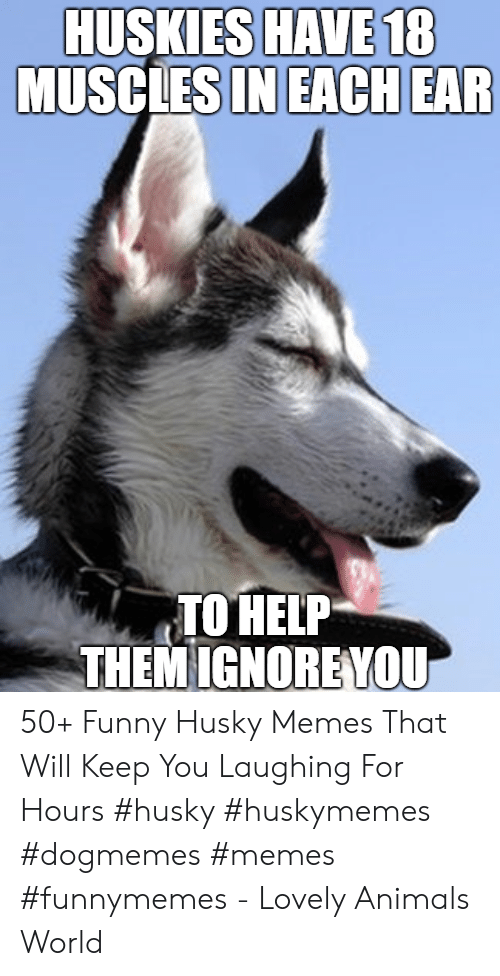
\includegraphics[width=0.4\textwidth,trim=0cm 10cm 0cm 0cm,clip=true]{husky2.png}
\caption{\label{fig:dogs} Welcome to the wonderful world of sled dogs.}
\end{figure}
By the way, force is also a vector, and we'll return to that later.
\end{frame}

\begin{frame}{Summary of force, work, and vector navigation}
Work required to raise one's altitude against force of gravity, $F = mg$:
\begin{equation}
W = m g d
\end{equation}
How many Joules would it take to hike up a mountain that is 4000 m tall (approximately), if you have a mass of 60 kg?  (\textbf{Work this one at your tables.})
\end{frame}

\section{Activity: Antarctic Maze}

\begin{frame}{Summary of force, work, and vector navigation}
(See handout).  The goal of this activity is to summarize our knowledge of the physics of navigation through polar environments.
\end{frame}

\section{Science lecture: Radio-glaciology, an Introduction.}

\end{document}
